%% This is an example first chapter.  You should put chapter/appendix that you
%% write into a separate file, and add a line \include{yourfilename} to
%% main.tex, where `yourfilename.tex' is the name of the chapter/appendix file.
%% You can process specific files by typing their names in at the 
%% \files=
%% prompt when you run the file main.tex through LaTeX.
\chapter{Project Management}

\section{Planning}

The project started with full-time dedication in September 2013 and was planned to be finished by December 2nd, 2013. The first steps were to study its feasibility in terms of technology, to outline the vision and specify the requirements with CREAF. Next steps included the design and implementation of the identified major components of the solution. It would end with the infrastructure setup, testing and the writing of the current document.

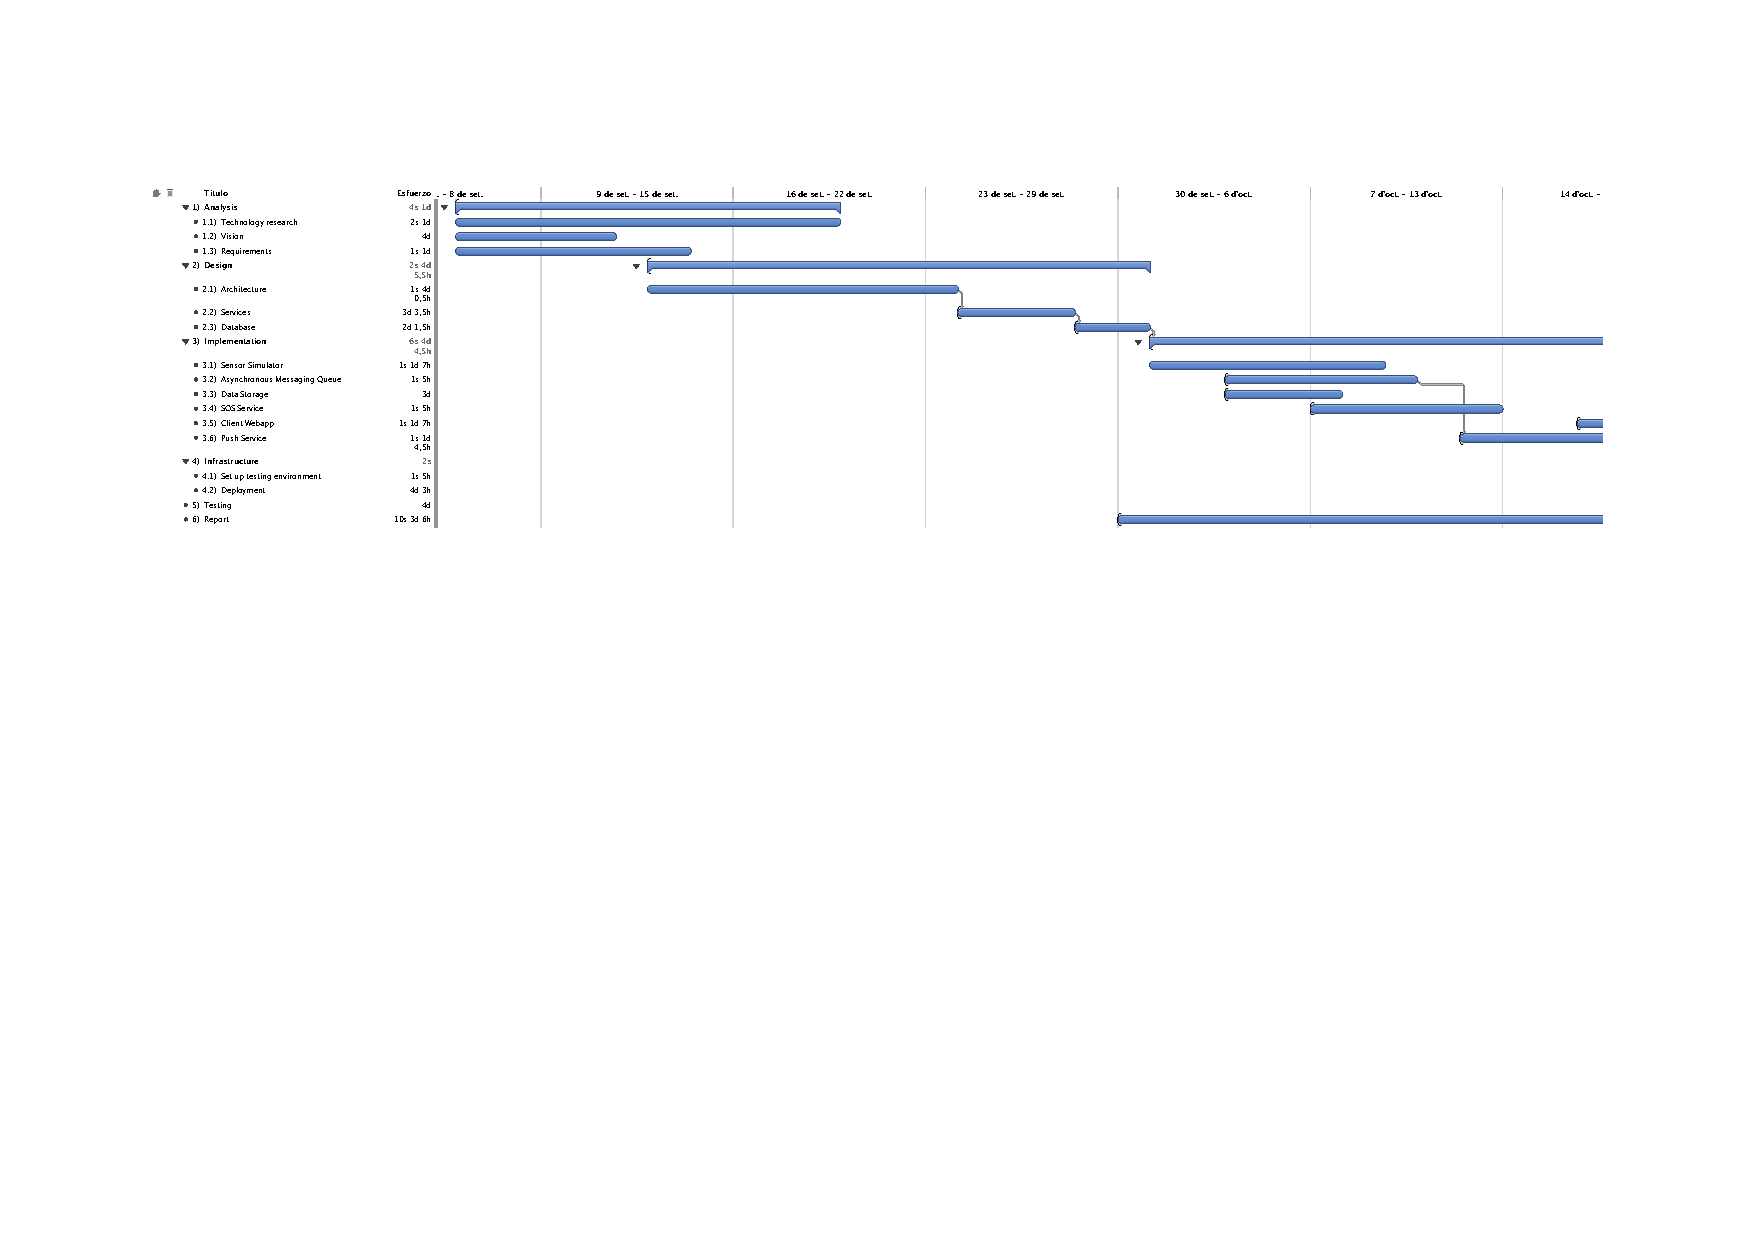
\includepdf[landscape=true, pages={1-2}]{initial_planning}

\section{Cost}

\subsection*{Human Resources}

The human resources involved in the project must be considered in order to forecast the costs of the project. These are an analyst who will be in charge of the Analysis and Design, a Developer who will implement the design and a System administrator who will set up the infrastructure. Therefore, considering these human resources and the initial planning, the overall cost is $15250\euro{}$, as detailed below.

\begin{table}[H]
    \centering
    \begin{tabular}{|l|c|c|r|}
    \hline
    \textbf{Resource}  & \textbf{Cost/Hour}  & \textbf{Hours}  & \textbf{Cost} \\ \hline
    Analyst            & 40\euro{}/h         & 200             & 8000\euro{}   \\ \hline
    Developer          & 25\euro{}/h         & 250             & 6250\euro{}   \\ \hline
    SysAdmin           & 20\euro{}/h         & 50              & 1000\euro{}    \\ \hline
    \textbf{Overall}   &                     &                 & \textbf{15250\euro{}} \\ \hline
    \end{tabular}
    \caption{Cost of human resources}
    \label{tab:human_cost}
\end{table}

Besides the time spent on the different stages of the development, additional time must be considered in order to write the current document. To that end, 90 additional hours plus the $200h + 250h + 45h = 495h$ invested by these human resources must be allocated, totalling $495h + 100h = 600h$.

\subsection*{Material Resources}

With regard to the software used in the development of the project, as all the frameworks, tools, code editors and languages have open-source licenses they don't involve any cost. Regarding the infrastructure, as it relies only on AWS free tier no cost is expected.

As for the development computer, the costs associated with its energy consumption plus its amortization must be taken into account. Being 1500€ the cost of computer and an amortization in 4 years, its cost per hour would the number of work hours in these years divided by its overall cost, $1500\euro / 8064h = 0.18\euro/h$. Considering that the power consumption of the computer is $64W/h$ and that the current price of the energy is about $0.20\euro/kWh$, the cost of the energy consumed by the computer is $0.064KW/h \times 0.20\euro/kWh = 0.0128\euro/h$. The overall cost of the material resources is detailed in the table below.

\begin{table}[H]
    \centering
    \begin{tabular}{|l|c|c|r|}
    \hline
    \textbf{Resource}   & \textbf{Cost/Hour}  & \textbf{Hours}  & \textbf{Cost} \\ \hline
    Computer            & 0.18\euro{}/h       & 600             & 108\euro{}   \\ \hline
    Energy              & 0.0128\euro{}/h     & 600             & 7,68\euro{}   \\ \hline
    \textbf{Overall}    &                     &                 & \textbf{115,68\euro{}} \\ \hline
    \end{tabular}
    \caption{Cost of material resources}
    \label{tab:material_cost}
\end{table}

Lastly, taking into account human and material resources the total cost of the project amounts $15250\euro + 115,68\euro = 15365,68\euro$.

\begin{table}[H]
    \centering
    \begin{tabular}{|l|c|}
    \hline
    \textbf{Resource}   & \textbf{Cost} \\ \hline
    Human               & 15250\euro{}   \\ \hline
    Material            & 115,68\euro{}   \\ \hline
    \textbf{Overall}    & \textbf{15365,68\euro{}} \\ \hline
    \end{tabular}
    \caption{Total cost of the project}
    \label{tab:total_cost}
\end{table}

\section{Execution}

Unfortunately, initial planning has suffered a few setbacks during its execution. It was first delayed at the beginning of December due to my need of finding a job and the time I spent working on a technical test required for a job offer. The major delay was caused by the impact the full-time job had in the dedication time, causing the project to be nearly stopped for several weeks. Although working on it occasionally, it was not until allocating 2 hours every day and full-time dedication on weekends that the project took effectively off. As a consequence, the planning for the remaining tasks was defined as follows.

Regarding the cost, AWS free tier provided not to be enough to fulfil the needs of the required infrastructure. Using three servers exceeded the maximum of 750 hours of EC2 micro instance usage. Thus, the overall cost has been 20.27\$ so far, missing the cost of June 2014. Assuming that the cost for both months was the same the total cost of the infrastructure would be $2 \times 20.27\$ = 40,54\$$, that is $29.92\euro$.

Moreover, another delay was encountered while executing this final planning. A disproportionately large Amazon AWS bill was received for what seemed to be either an attack on the system or a billing error. This required infrastructure to be shut down until the issue was resolved. Although having some impact, fortunately it didn't excessively affect planning.

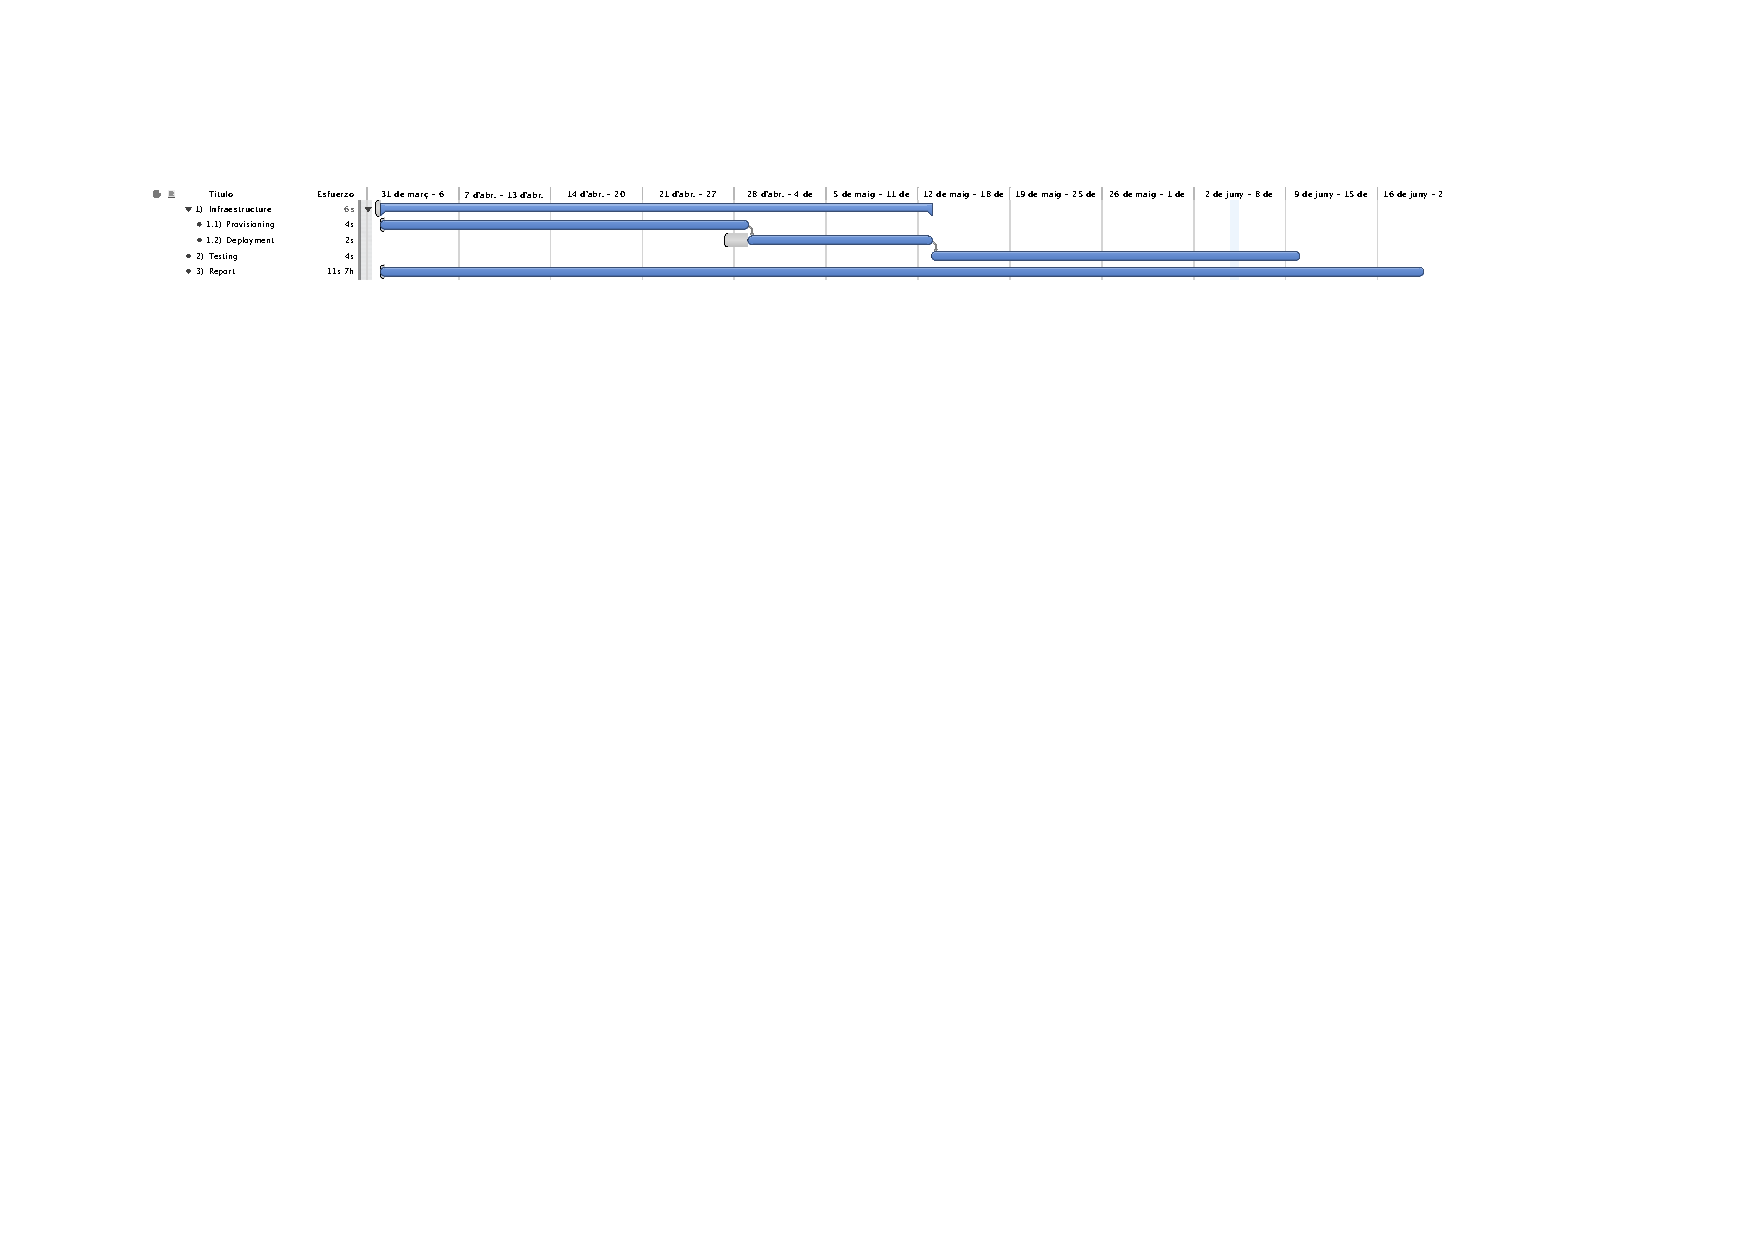
\includepdf[landscape=true, pages={1-2}]{final_planning}